%%%%%%%%%%%%%%%%%%%%%%%%%%%%%%%%%%%%%%%%%%%%%%%%%%%%%%%%%%%%%%%%%%%%%%%%%%%%%%%%
%2345678901234567890123456789012345678901234567890123456789012345678901234567890
%        1         2         3         4         5         6         7         8

\documentclass[letterpaper, 10 pt, conference]{ieeeconf}  % Comment this line out if you need a4paper
\usepackage{bbold}
\usepackage{xcolor}
\usepackage{hyperref}
\usepackage{graphicx}
\usepackage{booktabs}
\usepackage{colortbl}
\usepackage{ragged2e}
\usepackage{german}
%\selectlanguage{\german}
\selectlanguage{\english}
\usepackage{subfig}
%\usepackage[acronym]{glossaries}

%\usepackage{glossaries}

%\usepackage{biblatex}
%\{references.bib}

%\newacronym{GNN}{GNN}{global nearest-neighbour}
%\newacronym{RFS}{RFS}{Random Finite Sets}

%\define\gls{asd}

\def\andothers{\textit{et al.\xspace}}


%\documentclass[a4paper, 10pt, conference]{ieeeconf}      % Use this line for a4 paper

\IEEEoverridecommandlockouts                              % This command is only needed if 
                                                          % you want to use the \thanks command

\overrideIEEEmargins                                      % Needed to meet printer requirements.

% See the \addtolength command later in the file to balance the column lengths
% on the last page of the document

% The following packages can be found on http:\\www.ctan.org
%\usepackage{graphics} % for pdf, bitmapped graphics files
%\usepackage{epsfig} % for postscript graphics files
%\usepackage{mathptmx} % assumes new font selection scheme installed
%\usepackage{times} % assumes new font selection scheme installed
%\usepackage{amsmath} % assumes amsmath package installed
%\usepackage{amssymb}  % assumes amsmath package installed

\title{\LARGE \bf
Report about our work - data modelling
}


\author{
Jonas Munch {\tt\small j.munch@campus.fct.unl.pt} \\
Dusan Zeliar {\tt\small d.zeliar@campus.fct.unl.pt}
}

\begin{document}

\maketitle
\thispagestyle{empty}
\pagestyle{empty}

% TODO list:
% - Note density form of p(OperatorScore | TrackClass)


%%%%%%%%%%%%%%%%%%%%%%%%%%%%%%%%%%%%%%%%%%%%%%%%%%%%%%%%%%%%%%%%%%%%%%%%%%%%%%%%
\begin{abstract}
This technical report describes our work of the Data Modelling class 2017.
The goal of this work is to implement a tool that supports the user to transform a relational schemed database (OLTP) into a dimensional model (OLAP).
Based on an approach proposed by Moody %TODO ref
a so called star schema will be produced out of an arbitrary database.

The program guides the user via commandline interface through all the neccessary steps to find an agreement of which tables are selected as transaction entities, component entities and classification entities.

% TODO eventually add Aggregation operator

As soon as the selection phase is done, our software will generate a dimensional model based on the input scheme and populate it from the original data.

\end{abstract}


%%%%%%%%%%%%%%%%%%%%%%%%%%%%%%%%%%%%%%%%%%%%%%%%%%%%%%%%%%%%%%%%%%%%%%%%%%%%%%%%
\section{Introduction}
\label{sec:introduction}

\input{01introduction.tex}

\section{State of the Art}
\label{sec:related_work}

Klassifikation von Mustern wurde beschrieben in \cite{Niemann2007KVM}

\begin{figure}[tb]
  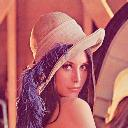
\includegraphics[width=0.8\linewidth]{images/lena}
  \caption{Lena}\label{f:lena}
\end{figure}

Jedes Bild sollte auch im Text erwähnt werden, so z.\,B.\ \figurename~\ref{f:lena}.



\section{Experiments}
\label{sec:experiments}

\input{03experiments.tex}

\section{Conclusion}
\label{sec:conclusion}

In this project, we implemented and tested creation of a basic dimensional model from Entity Relationship model. After studying existing methods of creating dimensional models we proposed an application. The application work flow starts with getting source database schema, suggesting a classification of entities and identifying hierarchies in model. The next step is collapsing hierarchies and aggregating data. Finally a new dimensional model database is created and the data is migrated. 	The created dimensional database is in a form of a star schemas, each start consists of a fact table and its dimensions. The schema shares the same dimensions between fact tables but does not contain connection between fact tables.
	The developed application can be extended by a connection between facts table to contain full star scheme of source database.
  


\addtolength{\textheight}{0cm}   % This command serves to balance the column lengths
                                  % on the last page of the document manually. It shortens
                                  % the textheight of the last page by a suitable amount.
                                  % This command does not take effect until the next page
                                  % so it should come on the page before the last. Make
                                  % sure that you do not shorten the textheight too much.

%%%%%%%%%%%%%%%%%%%%%%%%%%%%%%%%%%%%%%%%%%%%%%%%%%%%%%%%%%%%%%%%%%%%%%%%%%%%%%%%



%%%%%%%%%%%%%%%%%%%%%%%%%%%%%%%%%%%%%%%%%%%%%%%%%%%%%%%%%%%%%%%%%%%%%%%%%%%%%%%%



%%%%%%%%%%%%%%%%%%%%%%%%%%%%%%%%%%%%%%%%%%%%%%%%%%%%%%%%%%%%%%%%%%%%%%%%%%%%%%%%
\section*{Acknowledgment}


%%%%%%%%%%%%%%%%%%%%%%%%%%%%%%%%%%%%%%%%%%%%%%%%%%%%%%%%%%%%%%%%%%%%%%%%%%%%%%%%

\bibliographystyle{plain}
\bibliography{references}

\end{document}
